\newpage
\appendix
\section{Appendix}

\subsection{Proof of consistency theorem}
\label{appendix:theorem_proof}

Proof of the theorem in \ref{sec:theorem}:


\begin{theorem}[B2B consistency - general case]

     Consider the B2B model from equation \ref{eq:model} $$Y = (XS + N)F$$ with
     $N$ centered and full rank noise.

     If $F$ and $X$ are full-rank on $Img(S)$, then, the solution of B2B, $\hat
     H$ minimizes

     $$\min_H  \left \| X - XH\right\| ^2  + \left \| NH\right \| ^2$$ and satisfies

     $$S\hat H = \hat H$$
\end{theorem}
\begin{proof}

 Let $\hat G$ and $\hat H$ be the solutions of the first and second regressions
 of B2B.

 Since $\hat G$ is the least square estimator of $X$ from $Y$
 \begin{align*}
    \hat G = \arg \min_G \mathbb{S}[\left \| YG - X \right \|^2]
\end{align*}
Replacing $Y$ by its model definition $Y = (XS+N)F$, we have
 \begin{align*}
    \hat G &=   \arg \min_G \mathbb{S}[\left \| X - (XS + N)FG \right\|^2] =\arg \min_G \mathbb{S}[\left \| X - XSFG + NFG \right\|^2]
  \end{align*}
  Since $N$ is centered and independent of $X$, we have
  \begin{align}
    	  \hat G &=  \arg \min_G \left \| X - XSFG\right\| ^2  + \left \| NFG\right \| ^2
     \label{eq:Gdoublenorm}
\end{align}

In the same way, for $\hat H$, we have
\begin{align*}
    \hat H = \arg \min_H \mathbb{S}[\| XH - Y \hat{G} \|^2] &=\arg  \min_H \mathbb{S}[\| XH - (XS + N)F \hat G \|^2] \\
    &=\arg \min_H \mathbb{S}[\| X(H - SF \hat G) \| ^2] + \mathbb{S}[\| NF\hat G \| ^2]\\
    &= \arg \min_H \mathbb{S}[\| X(H - SF \hat G) \| ^2]
 \end{align*}
 a positive quantity which reaches a minimum (zero) for
 \begin{align}
    \hat H = SF \hat G
    \label{eq:Hdoublenom}
\end{align}

Let us now prove that $SF\hat G = F\hat G$.

Let $F^\dagger$ be the pseudo inverse of $F$, and $Z=F^\dagger SF\hat G$, we
have $FZ = FF^\dagger SF \hat G$

Since $F$ is full rank on $Img(S)$, we have $FF^\dagger S =S$, and $FZ = SF\hat
G$

As $S$ is a binary diagonal matrix, it is an orthogonal projection and therefore
a contraction, thus
 $$ \| NSF\hat G\|^2 \leq \| NF\hat G \|^2$$ and
 $$\left \| X - XSFZ\right \| ^2  + \left \| NFZ\right \| ^2 = \| X - XSF\hat G \| ^2  + \| NSF\hat G \| ^2 \leq \| X - XSF\hat G \| ^2  + \| NF\hat G \| ^2$$

But since $\hat G =  \arg \min_G \left \| X - XSFG\right\| ^2  + \left \| NFG\right \| ^2$, we also have
$$\left \| X - XSF\hat G\right\| ^2  + \left \| NF\hat G\right \| ^2 \leq \left \| X - XSFZ\right \| ^2  + \left \| NFZ\right \| ^2$$

Summarizing the above,
$$\left \| X - XSF\hat G\right\| ^2  + \left \| NF\hat G\right \| ^2 \leq \| X - XSF\hat G \| ^2  + \| NSF\hat G \| ^2 \leq \| X - XSF\hat G \| ^2  + \| NF\hat G \| ^2$$
$$\left \| X - XSF\hat G\right\| ^2  + \left \| NF\hat G\right \| ^2 = \| X - XSF\hat G \| ^2  + \| NSF\hat G \| ^2$$
$$\left \| NF\hat G\right \| ^2 =  \| NSF\hat G \| ^2$$

$N$ being full rank, this yields $SF\hat G = F\Hat G$.

Replacing into $\eqref{eq:Gdoublenorm}$, and setting $H = SFG$, we have
\begin{align*}
	\hat G &=  \arg \min_G  \left \| X - XSFG\right \| ^2  + \left \| NFG\right \| ^2 \\
	&=   \arg \min_G \left \| X - XSFG\right \| ^2  + \left \| NSFG\right \| ^2 \\
	\hat H &=  \arg \min_H \left \| X - XH\right \| ^2  + \left \| NH\right \| ^2
	\label{eq:4}
\end{align*}

Finally, $S\hat H = S SF\hat G = SF\hat G = \hat H$, since $S$, a binary
diagonal matrix, is involutive. This completes the proof.
\end{proof}



\newpage
\subsection{Modeling measurement noise}

Equation \ref{eq:model} does not explicitly contain a measurement noise term.
Yet, in most experimental cases, the problem is best described as:
\begin{equation}
  Y = (XS+N)F+M
  \label{eq:model_noisy_measure}
\end{equation}
  with $M\in \mathbb{R}^{m \times d_y}$.

This equation is actually equivalent to Equation \ref{eq:model} given our
hypotheses. Indeed, we can rewrite $M = MF^{-1}F$ over $Img(F)$, which leads to:
$$Y = (XS+N)F+M = (XS+N+MF^{-1})F = (XS+N')F$$

Consequently, assuming that $F$ is full rank on $Img(XS)$, B2B yields the same
solutions to equations \ref{eq:model} and \ref{eq:model_noisy_measure}.


\subsection{Feature importance}
\label{appendix:feature_importance}

For B2B, feature importance is assessed as follows:

\begin{algorithm}[H]
    %\SetAlgoLined
    \KwIn{$X_{train} \in \mathbb{R}^{m \times d_x}$, $X_{test} \in
\mathbb{R}^{m' \times d_x}$, $Y_{train} \in \mathbb{R}^{m\times d_y}$, $Y_{test}
\in \mathbb{R}^{m'\times d_y}$, } \KwOut{estimate of prediction improvement
$\Delta{R} \in \mathbb{D}^{d_x}$.} $H, G = \text{B2B}(X_{train}, Y_{train})$\;
$R_{full} = \text{corr}(X_{test} H, Y_{test} G)$\;

    \For{$i = 1, \ldots, d_x$}{ $K = Id$\; $K[i] \leftarrow 0$\;
    $R_{k} =
\text{corr}(X_{test} K H, Y_{test} G_i)$\; $\Delta R_i = R_{full} - R_{k}$\; }
\Return{$\Delta R$} \caption{B2B feature importance.} \label{algorithm:b2b_fi}
\end{algorithm}

For the Forward Model, the feature importance is assessed as follows:

\begin{algorithm}[H]
    %\SetAlgoLined
    \KwIn{$X_{train} \in \mathbb{R}^{m \times d_x}$, $X_{test} \in
\mathbb{R}^{m' \times d_x}$, $Y_{train} \in \mathbb{R}^{m\times d_y}$, $Y_{test}
\in \mathbb{R}^{m'\times d_y}$, } \KwOut{estimate of prediction improvement
$\Delta{R} \in \mathbb{D}^{d_x, d_y}$.}

$H = \text{LinearRegression}(X_{train}, Y_{train})\;
R_{full} = \text{corr}(X_{test} K, Y_{test})$\;

    \For{$i = 1, \ldots, d_x$}{ $K = Id$\; $K[i] \leftarrow 0$\; $R_{k} = \text{corr}(X_{test}
K H, Y_{test})$\; $\Delta R_i = R_{full} - R_{k}$\; } \Return{$\Delta R$}
\caption{Forward feature importance.} \label{algorithm:fwd_fi} \end{algorithm}

% \iffalse
% \begin{enumerate}
%   \item Fit $H$ given $X_{train}$ and $Y_{train}$
%   \item For each feature $i$:
%   \begin{itemize}
%     \item Define $K$, and identity matrix whose row $i$ has been zeroed-out
%     \item Fit $H^i_k$ given $X_{train} K$ and $Y_{train}$
%   \end{itemize}
%   \end{enumerate}
% \fi

For the CCA and PLS models, the feature importance is assessed as follows:

\begin{algorithm}[H]
    %\SetAlgoLined
    \KwIn{$X_{train} \in \mathbb{R}^{m \times d_x}$, $X_{test} \in
\mathbb{R}^{m' \times d_x}$, $Y_{train} \in \mathbb{R}^{m\times d_y}$, $Y_{test}
\in \mathbb{R}^{m'\times d_y}$, } \KwOut{estimate of prediction improvement
$\Delta{R} \in \mathbb{D}^{d_x, d_z}$.} $H, G = \text{CCA}(X_{train},
Y_{train})$\; $R_{full} = \text{corr}(X_{test} H, Y_{test} G)$\;

    \For{$i = 1, \ldots, d_x$}{ $K = Id$\; $K[i] \leftarrow 0$\; $R_{k} = \text{corr}(X_{test} K H,
Y_{test} G)$\; $\Delta R_i = R_{full} - R_{k}$\; } \Return{$\Delta R$}
\caption{CCA and PLS feature importance.} \label{algorithm:cdp_fi}
\end{algorithm}

For the Backward Model, feature importance cannot be assessed because there is
no prediction combining multiple factors.

\subsection{Recovering S}
\label{recovering}

In case of noise, B2B yields non binary $\hat S$. Three thresholding rules can
be used to binarize its values thus explicitly recover "causal" features.

First, given known signal-to-noise ratio, the threshold above which a feature
should considered to be "causal" can be derived analytically. Indeed, Equation
$\ref{eq:diagk}$ implies that the $k$ first diagonal elements of $\hat H$ are
bounded:  % we assume that $F$ has full rank over $Img(S)$.

$$0 \leq \frac{\sigma_{X_k}}{\sigma_{X_k} +\sigma_{N_1}} \leq
\text{diag}_k(\hat{H})\leq  \frac{\sigma_{X_1}}{\sigma_{X_1} +\sigma_{N_k}}$$
where $\sigma_{X_1}$, $\sigma_{X_k}$, $\sigma_{N_1}$ and $\sigma_{N_k}$ denote
the largest and smallest eigenvalues of $\Sigma_{X_1 X_1}$ and $\Sigma_{N_1
N_1}$.

The average value $\mu$ of non-zero coefficients of $\text{diag}(\hat H)$ is the
trace of $\hat H$ divided by $k$, and can be computed as
\begin{equation}
\mu = \frac{Var(X)}{Var(X)+Var(N)}
\end{equation}

The decision threshold between "causal" and "non-causal" elements is thus a fraction
$\mu$, whose proportion arbitrarily depends on the necessity to favor type I and
type II errors. In practice, we cannot use this procedure for our fMRI and MEG experiments,
because signal-to-noise ratio is unknown.

Second, $\text{diag}(\hat H)$ can be binarized with the Sonquist-Morgan
criterion \citep{sonquist_morgan}, a non-parametric clustering procedure
separating small and large values in a given set. This procedure maximizes the
ratio of inter-group variance while minimizing the intra-group variance, over
all possible splits of the diagonal into $p$ largest values and $d_x-p$ smallest
values. Let $m_0$ and $m_1$ be the average values of the two clusters, $p$ and
$d_x-p$ their size, and $v$ the total variance of the sample, Sonquist-Morgan
criterion maximizes \citep{kass75}:
\begin{equation}
  \frac{p(d_x-p)}{d_x} \frac{(m_1 - m_0)^2}{v}
\end{equation}

This procedure assumes that there exists at least one causal and at least one
non-causal feature.
%
Third, second-order statistics across multiple datasets can be used to identify
the elements of $\text{diag}(\hat H)$ that are significantly different from 0.
This procedure is detailed in the method section of our MEG experiment.

Overall, these three procedures thus vary in their additional assumptions: i.e.
(1) a known signal-to-noise ratio, (2) the existence of both causal and
non-causal factors or (3) independent repetitions of the experiment.

\section{Additional Figures}


% \begin{figure}[t!]
%   \centering
%   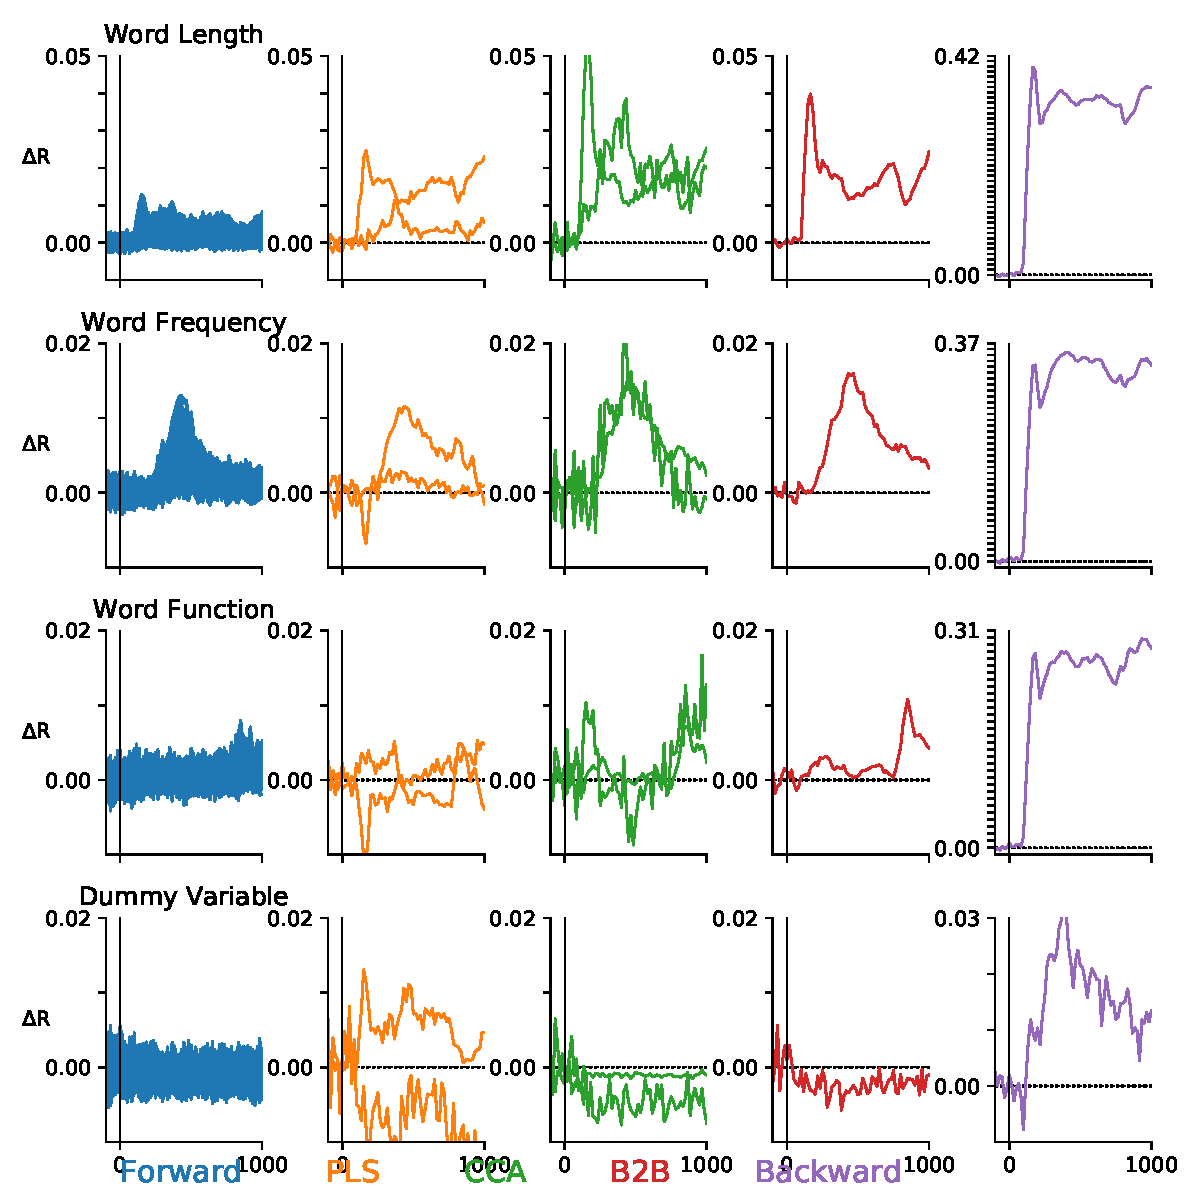
\includegraphics[width=\textwidth, trim=0cm 0cm 0cm 0cm, clip=True]{figures/meg_supp.pdf}
%   \caption{Average $\Delta R$ for each $Y$ dimension (Forward model), canonical components (PLS and CCA) or feature (B2B) across subjects. Formally, Backward model cannot have a $\Delta R$ because it never unmixes the multiple $X$ features. In such cases, we thus simply report the decoding score.}
%   \label{fig:meg_supp}
% \end{figure}


\begin{figure}
  \centering
  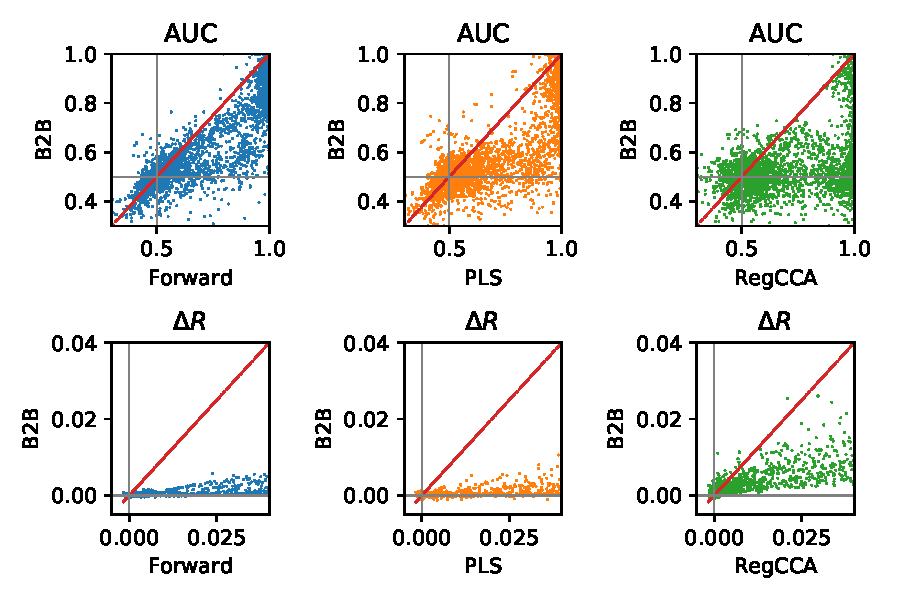
\includegraphics[width=\linewidth]{figures/delta_auc.pdf}
  \caption{Synthetic experiments. Distribution (over conditions) of AUC (top) and Feature
  Importance $\Delta R$ (bottom) metrics between our method (y-axis) and the baselines
  (x-axis). Each dot is a distinct synthetic experiment. Dots below the diagonal indicates
  that B2B outperform the tested model. \label{fig:auc_plots}}
\end{figure}

\begin{figure}
  \centering
  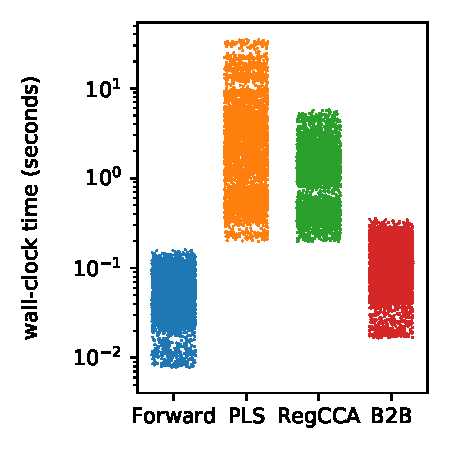
\includegraphics[width=0.7\linewidth]{figures/duration}
  \caption{Wall-clock run-time for our method B2B and for the baselines. Each dot is a
  distinct synthetic experiment. B2B runs much faster than cross-decomposition baselines.
  \label{fig:duration}}
\end{figure}

\subsection{Supplementary comparison of models' coefficients}

Following the recommendations of one of our reviewers, we implemented a
multivariate variant of the forward model, i.e. a MANOVA, using the statsmodels
implementation \citep{seabold2010statsmodels}. MANOVA is primarily used as a
inferential statistics, and does not trivially convert to a predicting method.
Consequently, we did not find a way to compare MANOVA against B2B with the
$\Delta R$ evaluation. However, the effects of MANOVA are generally summarized
with the Wilk's Lambda stastistics or its transformation into an $F$-value.
For each searchlight, we thus use the $F$-values of the
Wilk's Lambda statistics as proxy for $\hat S$ and feeds it to a second-level
Wilcoxon signed-rank tests across subjects, like we did for the other models.

The results show that all factors, including the Dummy variable, are
systematically above chance level in all recorded brain regions (Fig.~\ref{fig:fmri_supp}). This result
can be explained by the large dimensionality of $Y$. Indeed, limiting the
searchlight to a 1mm radius did not lead to these spurious effects but provided
results similar to the Forward model.

Nonetheless, MANOVA does appear to capture some plausible effects. Indeed, the
$F$-values obtained for both Word Length and Word Frequency were weakly but
significantly higher than those obtained with the Dummy variable in the
occipital and temporal brain areas (Fig.~\ref{fig:fmri_supp}). This results
suggests that the effect size of the MANOVA can be biased and, thus, is not
valid for second-level statistics.

Overall, this suggests that MANOVA (1) can lead to positively biased estimates of
$\hat S$ (2) appears weaker than B2B in terms of second-level analysis across
subjects (3) misses the effect of Word Function detected with the Forward model,
and (4) does not trivially translate into a prediction tool. Together these
elements thus suggest that MANOVA is less suitable to the present objective than
B2B.


\begin{figure}
  \begin{center}
    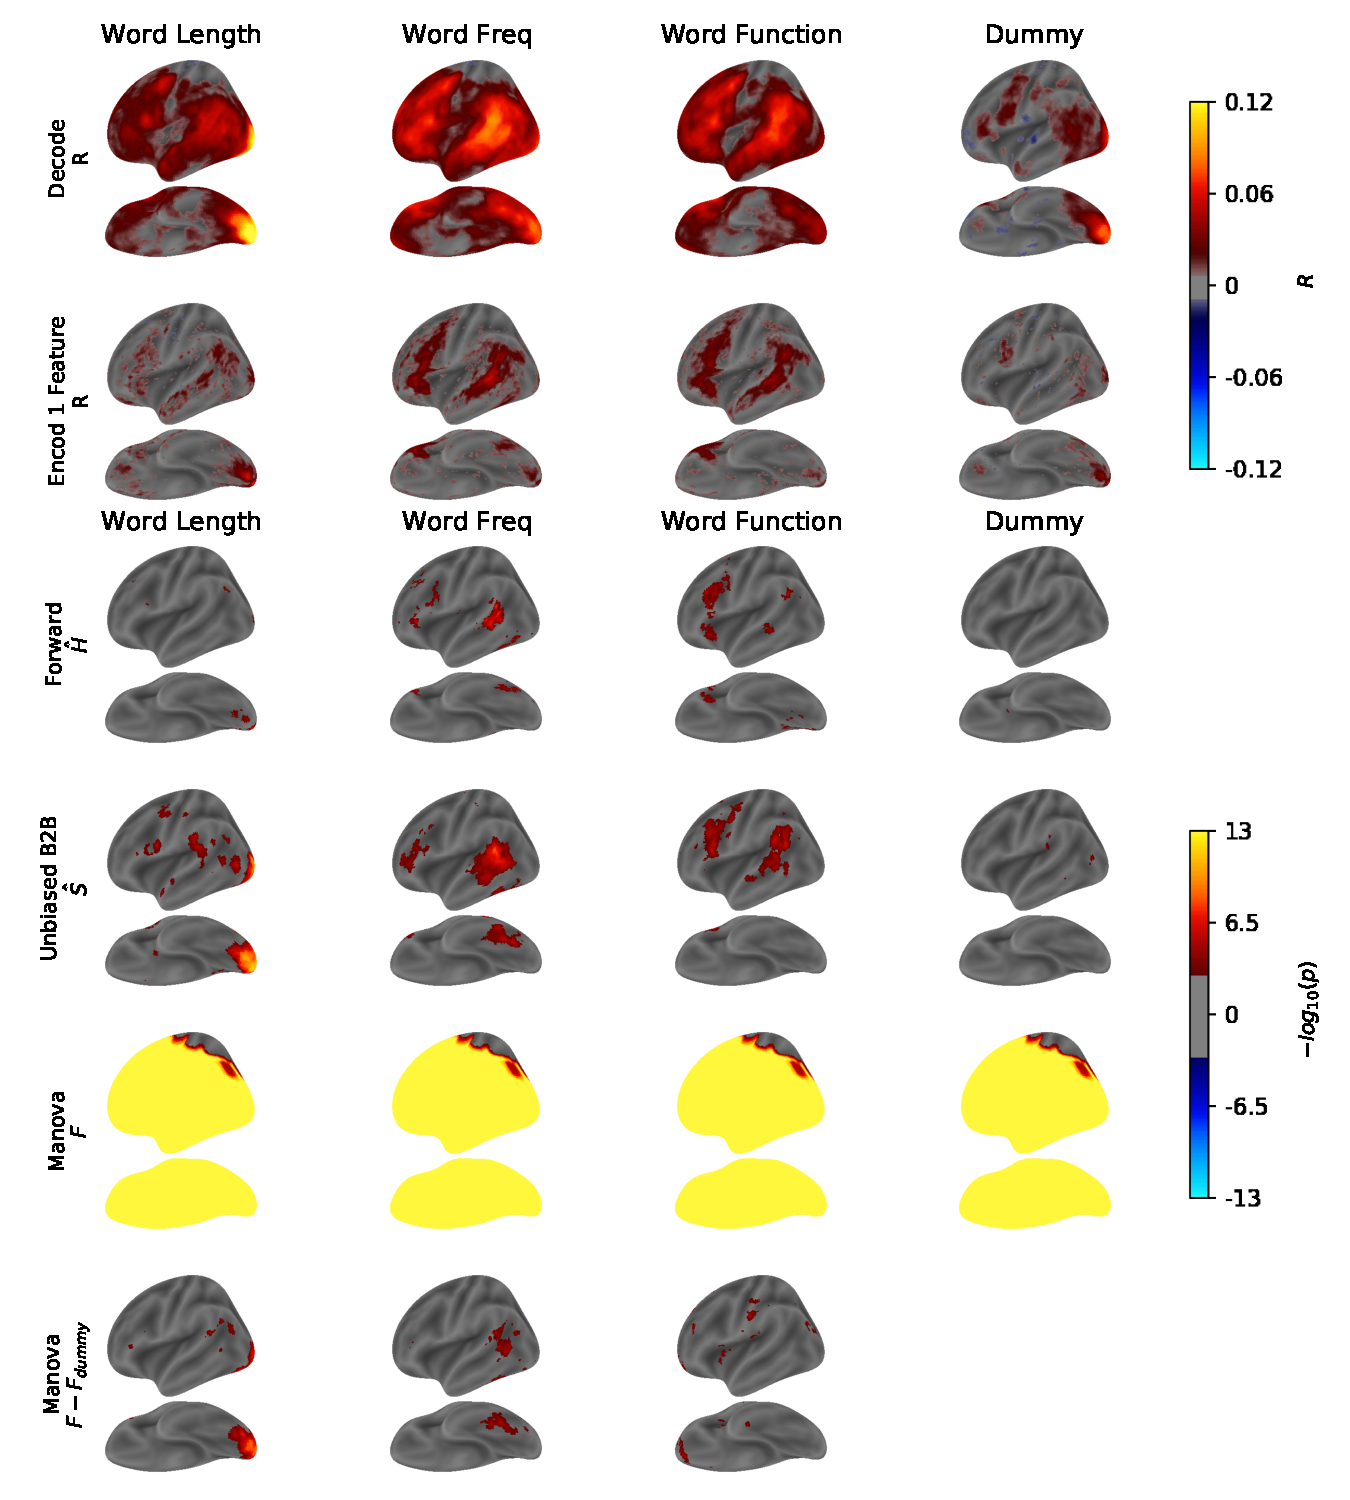
\includegraphics[width=0.7\textwidth,
                     trim=0cm 0cm 0cm 0cm,
                     clip=True]{figures/fmri_controls.pdf}

    \label{fig:fmri_supp}
  \end{center}
  \caption{Top two rows. Pearson $R$ correlation obtained for a Backward decoding model and
  a Forward encoding model trained with one factor at a time. These models can
  not take into account the factor covariance, and thus lead to spurious effects
  (e.g. visual cortex effect for the dummy variable). Bottom five rows. Second-
  level p-values across subjects for the coefficients of the Forward, a B2B and a Manova trained with
  all factors, as well as for the $\Delta R$ of the B2B, for comparison.
  B2B achieves better p-values, without leading to spurious effects for
  the Dummy variable. The Manova leads to biased estimates due to its inability
  to deal with overfitting. The last row shows where the Manova's $F$-values of each factor differs
  significantly from the $F$-values estimated for the Dummy variable.}
\end{figure}

\subsection{Robustness to increasing number of factors}

To test whether each of the methods robustly scales to an increasingly
large number of potential causes $X$, we enhanced the four ad-hoc features
(word length, word frequency, word function, dummy variable) with another
ten features. These additional features corresponds to the first dimensions
of word embedding as provided by Spacy \citep{spacy2}. The MEG results shown
in Fig.~\ref{fig:embeddings}, show that the feature importance of ad-hoc
features as derived by B2B remain unchanged and are actually improved.

\begin{figure}
  \centering
  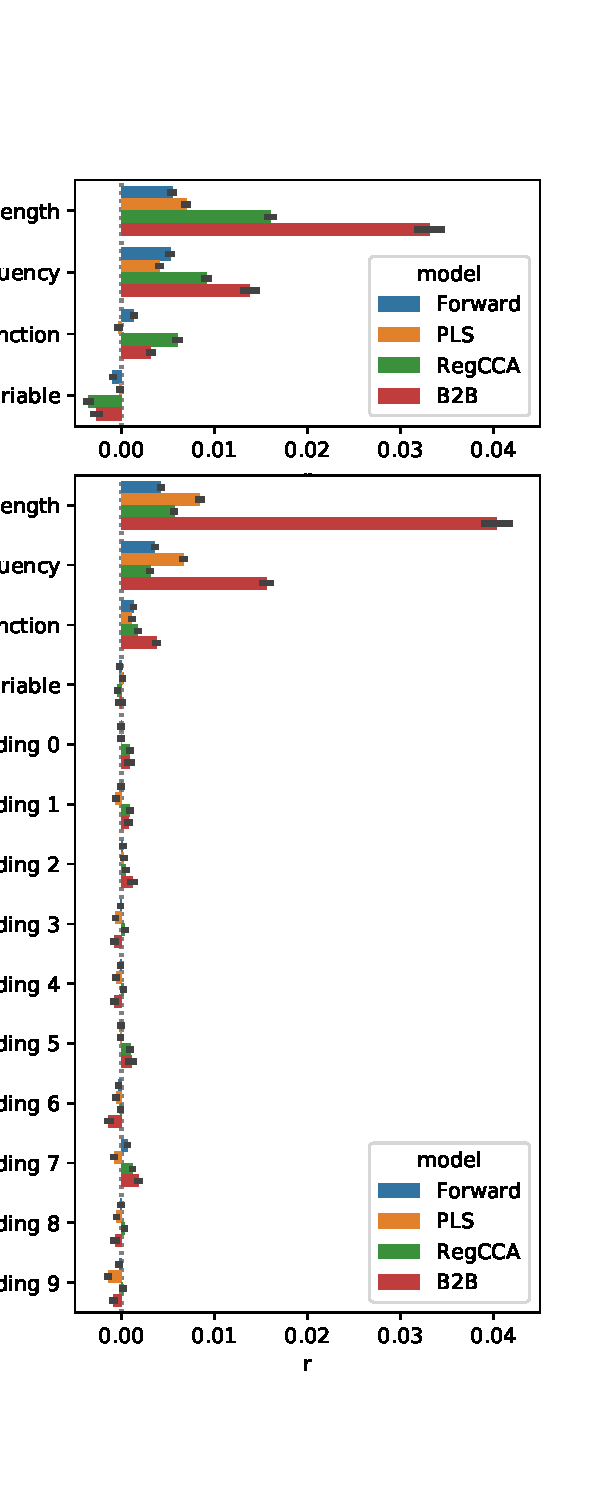
\includegraphics[width=0.5\linewidth]{figures/compare_embeddings.pdf}
  \caption{Comparison of $\Delta R$ when the models are tested on four
  variables (top) and when the models are tested on an these four variables
  as well as another 10 word-embedding features (bottom). These results
  illustrate that, unlike Regularized CCA, B2B remains robust even when
  the number of tested factors increases.
  \label{fig:embeddings}}
\end{figure}
